\documentclass[10pt]{beamer}



%%%
% PREAMBLE FOR THIS DOC 
%%%
%https://tex.stackexchange.com/questions/68821/is-it-possible-to-create-a-latex-preamble-header
\usepackage{/Users/miw267/Repos/csci246_spring2025/slides/preambles/beamer_preamble_for_CSCI246}

\usepackage{wrapfig}  


%%% TRY TO RESHOW TOC AT EACH SECTION START (with current section highlighted)
% Reference: https://tex.stackexchange.com/questions/280436/how-to-highlight-a-specific-section-in-beamer-toc
\newcommand\tocforsect[2]{%
  \begingroup
  \edef\safesection{\thesection}
  \setcounter{section}{#1}
  \tableofcontents[#2,currentsection]
  \setcounter{section}{\safesection}
  \endgroup
}


\usepackage[normalem]{ulem} % for strikeout (\sout)

%%%% HERES HOW TO DO IT CORRECTLY
% FIRST IN .STY FILE, DO
%\usetheme[sectionpage=none]{metropolis}
% THEN AT EACH SECTION DO
%\begin{frame}{Outline}
%  \tableofcontents[currentsection]	
%\end{frame}



%\setbeamertemplate{navigation symbols}{}
%\setbeamertemplate{footline}[frame number]{}


%%%
% DOCUMENT
%%%

\begin{document}

%\maketitle

%% Title page frame
%\begin{frame}
%    \titlepage 
%\end{frame}



\title{03/03/2026: It\^{o} Integration}
\author{CSCI 546: Diffusion Models}
\date{Textbook reference: Chang Sec 6.9-6.11, GS Sec  13.8-13.9}

\begin{frame}
    \titlepage 
\end{frame}

\begin{frame}

\begin{mygreenbox}[title=Announcement (Sign-in Sheet)]
Please sign the sign-in sheet.
\end{mygreenbox}

\vfill 


\begin{myredbox}[title=Announcement (Office Hours Before Midterm)]
\begin{itemize}
\item Today, 12:15pm-1:15pm, Barnard 352 \textbf{or} Wilson.
\item Tomorrow (Extra), 2pm-4pm Barnard 352. 	
\end{itemize}

\end{myredbox}

\vfill 

\begin{myyellowbox}[title=Midterm Study Guide]
The midterm study guide is now complete, including all questions to study for the midterm.
\end{myyellowbox}
	
\end{frame}

\begin{frame}[standout]
Review Problem Set \#13
\end{frame}

\begin{frame}[standout]
Concepts for Problem Set \#14
\end{frame}


%\begin{frame}[standout]
%Outline for today's material
%\begin{itemize}
%\item \textbullet \quad \alert{Interpreting a Stochastic Differential Equation (SDE)}
%\item \textbullet \quad Difficulties with Integrating Against Brownian Motion
%\end{itemize}
%
%\end{frame}

\begin{frame}{Review: It\^{o} SDEs}

\small 

\fbox{%
\begin{minipage}{\linewidth}
\colorbox{blue!30}{\textbf{Definition.}} A SDE for the diffusion process $X$ with drift coefficient $\mu(x,t)$ and diffusion coefficient $\sigma(x,t)$ is
\[
dX(t)
=
\underbrace{
\colorbox{green!20}{$\mu(X,t)\,dt$}
}_{\text{\color{green!70!black} drift term}}
\;+\;
\underbrace{
\colorbox{red!20}{$\sigma(X,t)\,dW(t)$}
}_{\text{\color{red!70!black} diffusion term}}
\]
where $W$ is standard Brownian motion. 
\end{minipage}
	
}

\vfill
\only<2->{
\colorbox{yellow!30}{\textbf{Poll.}} Why it is common to model random continuous systems (e.g. the stock market) by integrating \alert{specifically} against Brownian motion $W$?
}
\vfill 
\only<3->{\colorbox{blue!30}{\textbf{Observations.}}}
\begin{enumerate}
	\item  \uncover<3->{
	\,
	\begin{quotation}
	If the noise in the system is due to a multitude of independent random changes, then the Central Limit Theorem predicts the net result will have the normal distribution, a property shared by the increments $W(t)-W(s)$ of the Wiener process.
\end{quotation}
\hfill \scripttext{- Brezezniak and Zastawniak (2000), \textit{Basic Stochastic Processes} pp. 151.}} 
\uncover<4->{\item Our definition implicitly restricts to \alert{It\^{o} SDEs}; there are also more general (non-It\^{o}) SDEs.}
\end{enumerate} 

\end{frame}


\begin{frame}{It\^{o} SDEs: Historical Example}
\colorbox{green!30}{\textbf{History.}} In 1900, Louis Bachelier wrote a ground-breaking paper modeling asset prices at the Paris Stock Exchange.  \\


\begin{center}
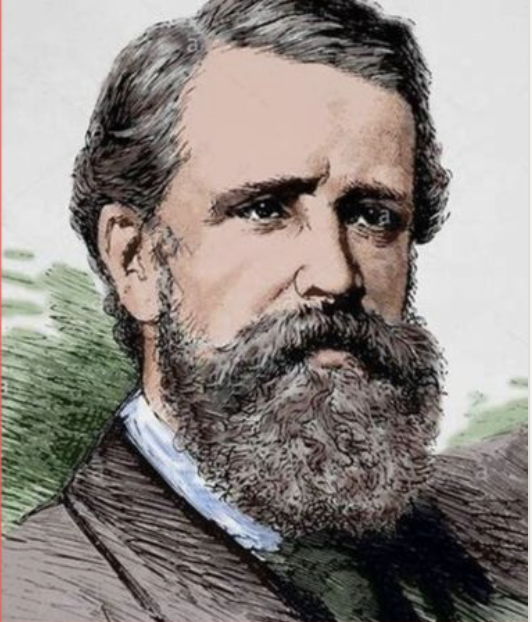
\includegraphics[width=.2\textwidth]{images/bachelier.png}
\end{center}

\pause 
He assumed infinitesimal price increments $dX(t)$ are proportional to the increments $dW(t)$ of Brownian motion
\[ dX(t) = \sigma dW(t),\]
where $\sigma$ is a positive constant.
\pause 
As a result, an asset with an initial price $X(0)=x$ would be worth
\[ X(t) = x + \sigma W(t)\]
at time $t$.  \pause 


\bottomtext{\hfill Brezezniak and Zastawniak (2000), \textit{Basic Stochastic Processes} pp. 151.}
\end{frame}


\begin{frame}{It\^{o} SDEs: Historical Example}
\only<1->{
\colorbox{yellow!30}{\textbf{Poll.}} What do you think of Louis Bachelier's approach of modeling financial assets as
\[ dX(t) = \sigma dW(t) \qquad \qquad ? \]	
}

\vfill 

\only<2->{
\begin{center}
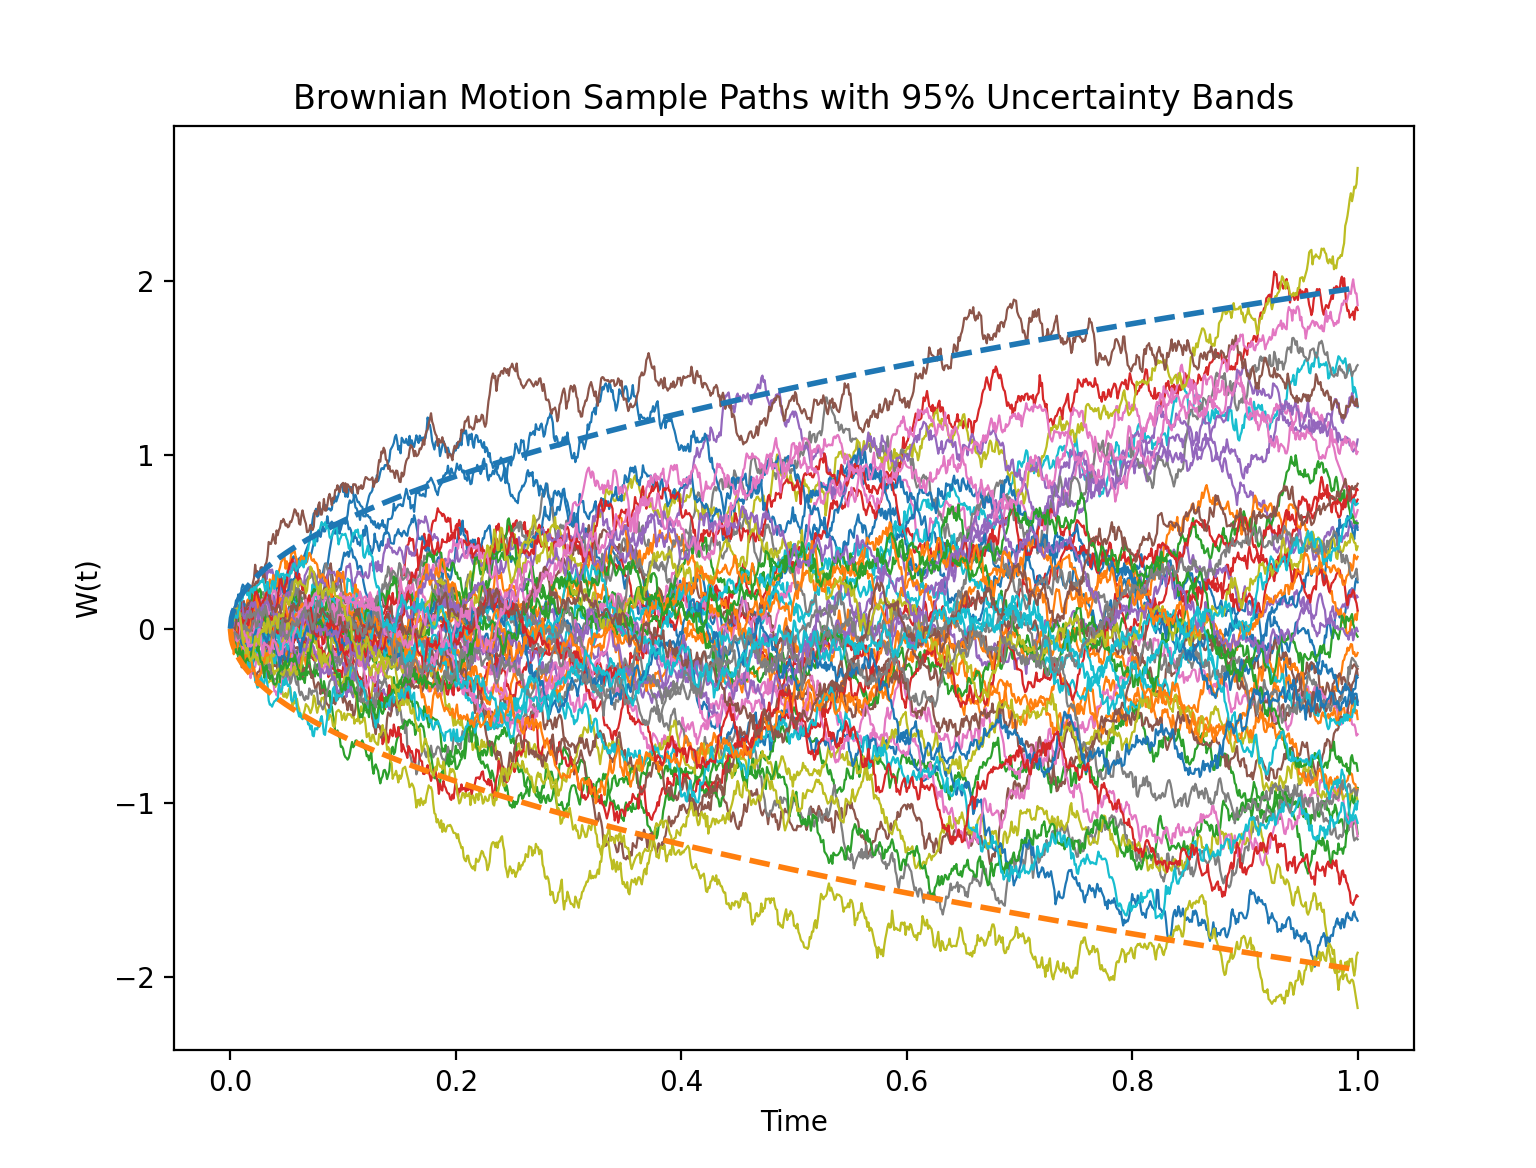
\includegraphics[width=.52\textwidth]{images/brownian_motion_sample_paths.png}
\end{center}
}

\vfill 
\only<3->{
\colorbox{blue!30}{\textbf{Observation.}} In this model, stock prices can go \alert{negative.}
} 

\only<4->{
In fact, $P(X_t <0) = \half$ at any time $t$.
}


\end{frame}


\begin{frame}{It\^{o} SDE Example: Geometric Brownian Motion}
A better approach is to have the potential gain or loss $dX(t)$ grow \alert{proportionally} to the invested sum $X(t)$:
\[ \frac{dX(t)}{X(t)} = \sigma \, dW(t)\]

\pause 
Or more generally,
\begin{align*}
 \frac{dX(t)}{X(t)} &= \mu \, dt + \sigma \, dW(t) \\
 \implies dX(t)&= \mu \, X(t) \, dt + \sigma \, X(t) \, dW(t)
\end{align*}
\pause 

This is known as \alert{\texttt{geometric Brownian motion.}}

\end{frame}


\begin{frame}{It\^{o} SDE Example: Geometric Brownian Motion}

\only<1-4>{
\begin{align*}
 dX&= \mu X \, dt + \sigma X \, dW
\end{align*}
}

\begin{center}
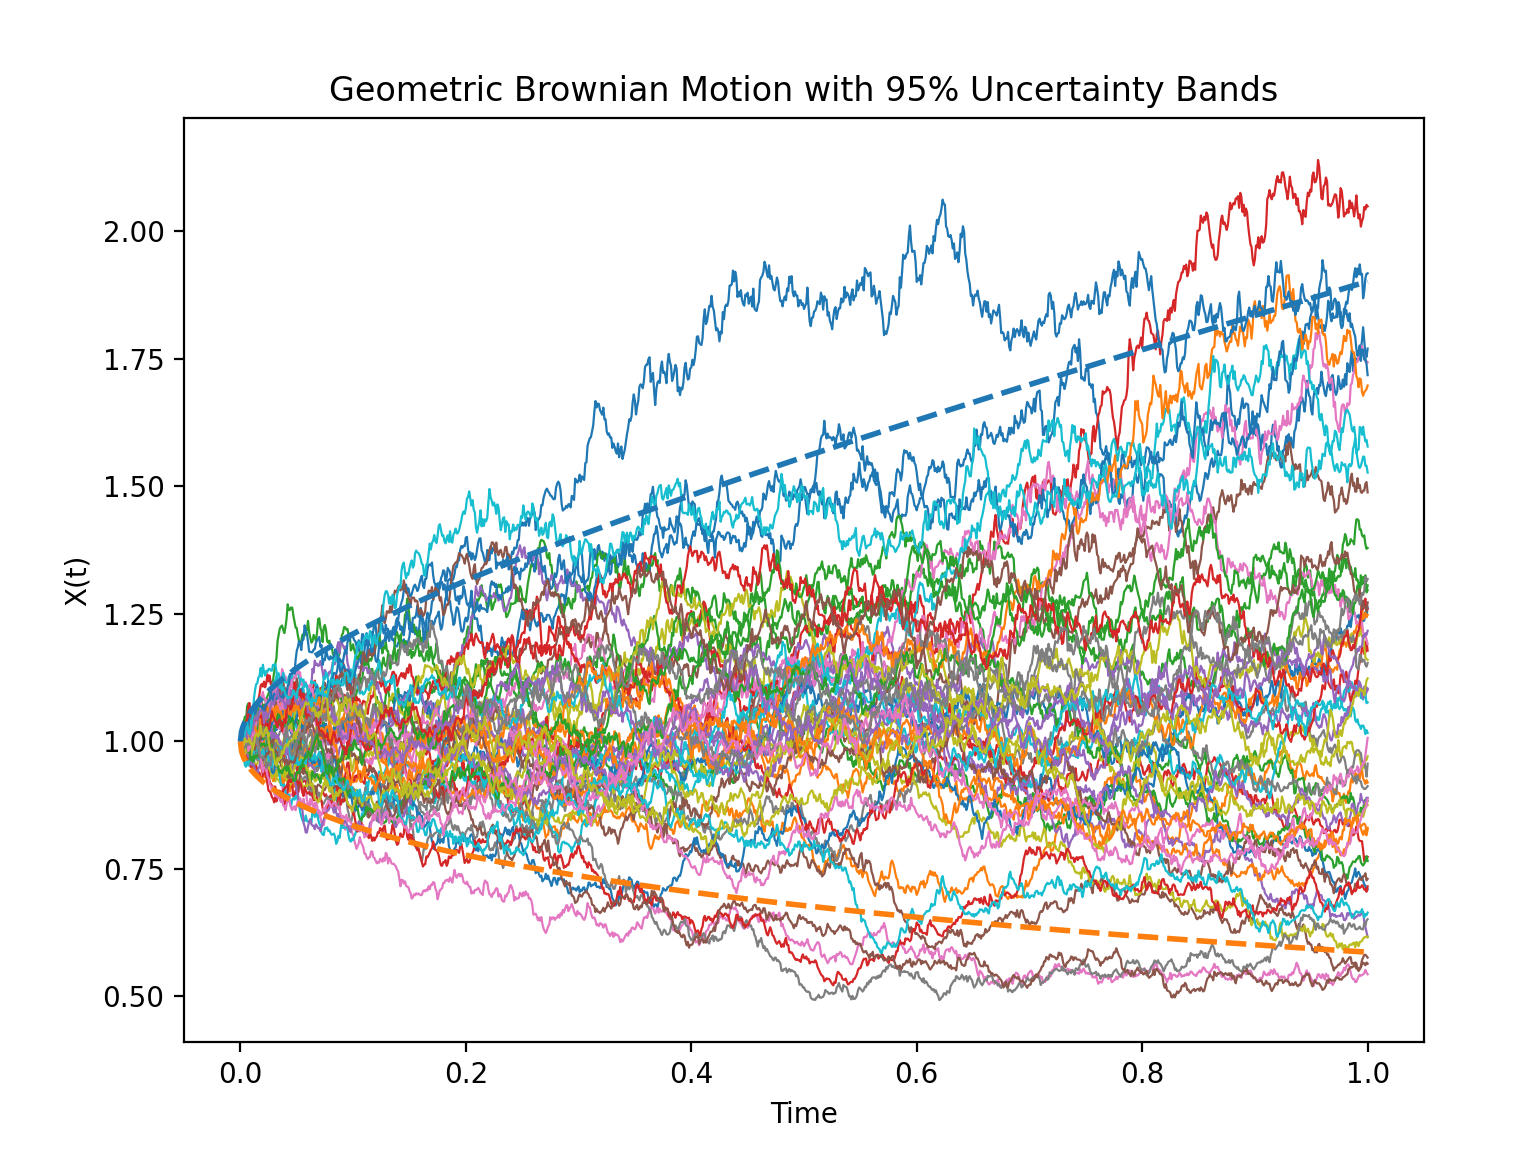
\includegraphics[width=.5\textwidth]{images/geometric_brownian_motion_sample_paths.png}
\end{center}

\only<2-4>{Now:
\begin{itemize}
\onslide<2-4>{\item  The sample paths are always positive.}
\onslide<3-4>{\item  The expected value grows exponentially over time $E[X_t]=X_0 e^{\mu t}$.}
\onslide<4>{ \item  The confidence bands widen exponentially over time.}
\end{itemize}
}

\only<5-6>{
Yet another way to describe geometric Brownian motion is
\begin{align*}
\colorbox{blue!15}{$Y_t=e^{X_t}$,}
\end{align*}
where $X_t$ satisfies the SDE $dX = \mu \, dt + \sigma \,  dW$ %(where $X_t$ satisfies the SDE $dX = a\, dt + \sigma \,  dW$ with $a= \mu - \half \sigma^2$).
} 

\vfill 
\only<6>{
The desire to \underline{compose} stochastic processes motivates the \alert{It\^{o} chain rule}, a chain rule for stochastic processes.
}



\end{frame}

\begin{frame}{It\^{o} chain rule} 

Let  $X(\cdot)$ be a 1-dimensional real-valued stochastic process which solves the following SDE, constructed from  1-dimensional Brownian motion $W$
%
\begin{align}
\forestgreen{dX = b \, dt + dW.}	
\label{eqn:SDE_with_one_dim_obs_and_brownian_motion}
\end{align}
\pause 
Let $u: \R \to \R$ be a given smooth function, $u=u(x)$.  What SDE does the SDE below solve?
\[ Y(t) \defeq u(X(t)), \qquad (t \geq 0) \]
\pause 
Intuitively, we would guess by chain rule that  
%
\begin{align}
dY = \frac{du}{dX}dX = u' \forestgreen{dX} = u' \forestgreen{b dt} + u' \forestgreen{dW}.
\label{eqn:intuitive_guess_at_sde_chain_rule}
\end{align}
where we use the notation ${}^\prime = \frac{d}{dx}$.
\pause 
%
%\footnotetext{where (1) heuristically applies the chain rule, (2) just introduces the notation ${}^\prime = \frac{d}{dx}$, and (3) just substitutes  \Eqref{eqn:SDE_with_one_dim_obs_and_brownian_motion}.}

However, \Eqref{eqn:intuitive_guess_at_sde_chain_rule} is wrong! \redx.   \pause Recall that Brownian motion is so irregular that its fluctuations scale with  the \textit{square root} of time increments:
%

\begin{align}
\colorbox{blue!15}{$dW \approx (dt)^{\half}.$}
\label{eqn:brownian_motion_fluctuates_with_the_square_root_of_increments_in_time}
\end{align}
\end{frame}


\begin{frame}{It\^{o} chain rule} 
\small 
The irregularity in \Eqref{eqn:brownian_motion_fluctuates_with_the_square_root_of_increments_in_time} means that we need to keep additional terms in the Taylor series expansion of the differential: \\
\vspace{.4cm}
%
\scalebox{0.85}{
\begin{minipage}{\textwidth}
\begin{align*}
dY &= u' dX + \half u'' (dX)^2 + \hdots && \scripttext{Taylor series} \\	
\onslide<2->{&= u' (b dt + dW) + \half u'' (b dt + dW)^2 + \hdots && \scripttext{Substitute \Eqref{eqn:SDE_with_one_dim_obs_and_brownian_motion}}} \\	 
\onslide<3->{& = \bigg(u'b + \red{\half u''} \bigg) dt + u' dW + \text{\{terms of order $dt^{3/2}$ and higher\}}  && \scripttext{See below}}
\end{align*}
\end{minipage}
}
%
\vfill 
\pause 
\onslide<4->{\colorbox{blue!30}{\textbf{Remarks.}}} 
\begin{itemize}
\onslide<4->{\item Note the extra term \enquote{\;\red{$\half u'' dt$}\;} not present in ordinary calculus.}   

\only<5>{\colorbox{yellow!30}{\textbf{Poll.}} Where does this term come from?}
\onslide<6->{\item This term comes from the relation
\begin{align*}
\colorbox{blue!15}{$dW \approx (dt)^{\half}.$}
\end{align*}}
\only<7>{\colorbox{yellow!30}{\textbf{Poll.}} Can anybody explain?}\only<8->{Specifically, by foiling the quadratic differential, we get terms $(dt^2, dtdW, dW^2) \approx (dt^2, dt^{3/2}, dt)$.  We only keep the final term after foiling and absorb the rest into the higher-order terms.}	
\onslide<9->{\item \raisebox{-0.2em}{
\includegraphics[height=1.2em]{images/fire}} tip: To do the group exercises, just remember the first line!}
\end{itemize}
\only<10>{\vfill \vfill \vfill \vfill \tiny Reference for this slide: Evans (2012). \textit{An introduction to stochastic differential equations.}  For a more technically precise  statement of It\^{o}'s Lemma, see Evans or Section 5 of Gautam Iyer's \textit{\href{https://www.math.cmu.edu/~gautam/sj/teaching/2021-22/944-scalc-finance1/pdfs/ch3-int.pdf} {\blue{Stochastic Integration. (Lecture notes.)}}}}
\end{frame}



\begin{frame}{Integrating Brownian motion against Brownian motion}
\small 
\colorbox{yellow!30}{\textbf{Poll.}}  Let's consider the stochastic integral
\[V(T) = \int_0^T W_t \, dW_t \qquad \qquad \]

How can we interpret this? 
\pause 

\colorbox{green!30}{\textbf{Interpretations.}}
\begin{itemize}
	\item \textit{Finance.} $V(T)$ is the total profit from a betting strategy where a person bets an amount proportional to one's current position/capital $W_t$. \pause 
	\item \textit{Mental health.}  $V(T)$ is the emotional dysregulation (or relapse risk accumulation) when the effect of new stress $dW_t$ depends on how stressed $W_t$ the person already is. \pause 
	\begin{itemize}
	\item \textit{Multiplicative risk accumulation.} In general, this can be seen as the simplest mathematical prototype for \textit{risk accumulation in a system where shocks matter more when the system is already strained.} \pause 
	\end{itemize}  
\end{itemize}

\pause 

\colorbox{red!30}{\textbf{Problem.}} How in the world do we \alert{compute} this integral?!

\end{frame}

\begin{frame}{It\^{o} chain rule: A simple application} 

In the group exercises, we'll use It\^{o}'s chain rule to verify the identity
\[ \int_0^T W \, dW = \half \bigg( W^2(T) - T \bigg). \]


\onslide<2->{\colorbox{blue!30}{\textbf{Remarks.}}} 
\begin{itemize}
\onslide<2->{\item In stochastic calculus, the result of the definite integral is a \alert{random variable}, not a \textit{number} as in ordinary calculus.} 
\onslide<3->{\item Also note the extra term \enquote{\;\red{$-T$}} not present in ordinary calculus.} 
\onslide<4->{\item Without this \enquote{It\^{o} correction term}, the integral is not correct, as can be verified by numerical simulations.} 
\end{itemize}
\end{frame}


\begin{frame}{Verifying the It\^{o} correction term} 
\begin{center}
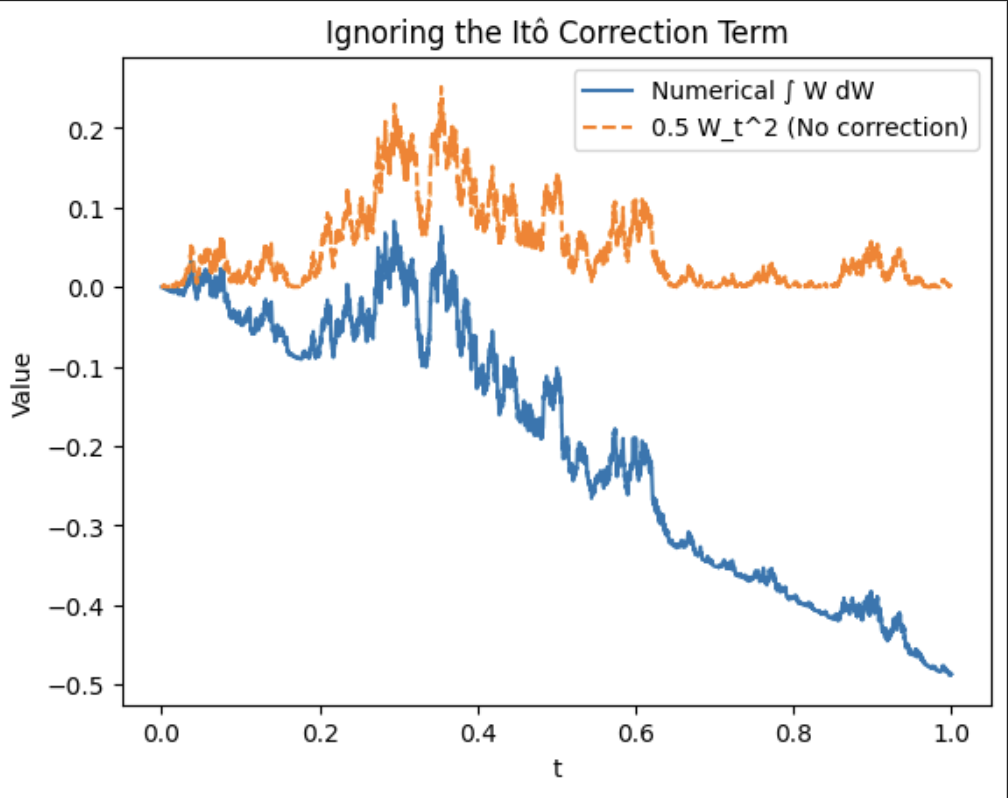
\includegraphics[width=.5\textwidth]{images/ito_correction_term_1.png} \\
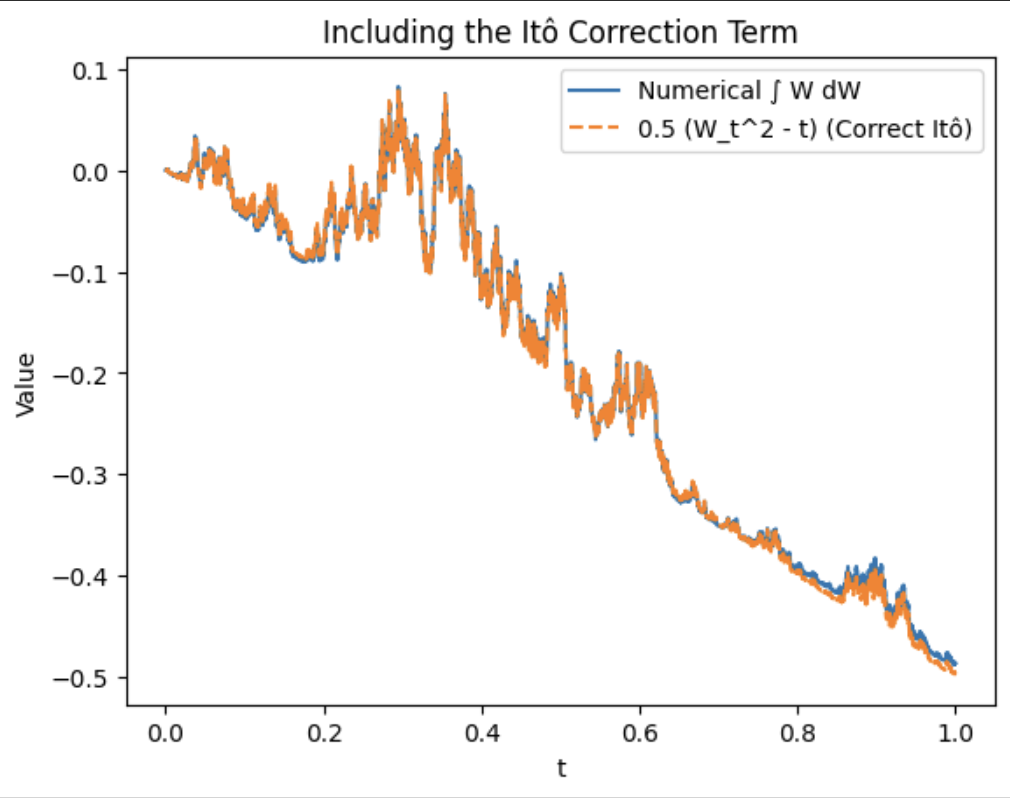
\includegraphics[width=.5\textwidth]{images/ito_correction_term_2.png}
\end{center}


\end{frame}



\begin{frame}{Verifying the It\^{o} correction term} 

\colorbox{yellow!30}{\textbf{Review.}} Recall that we could interpret the integral 
\[V(T) = \int_0^T W_t \, dW_t \qquad \qquad \]

as the total profit from a betting strategy where a person bets an amount proportional to one's current position/capital $W_t$. 
\vfill 
\colorbox{blue!30}{\textbf{Observation.}} This gives another corroboration of \red{It\^{o}'s correction term} $\int_0^T W_t \, dW_t = \half \big( W^2(T) \red{- T} \big)$: without it, there would be a way to make unlimited money by betting (arbitrage)!
	
\end{frame}




\begin{frame}{Random Groups}

\begin{columns}
\begin{column}{0.33\textwidth}
Aubrey Williams: 5 \\ 
Austin Barton : 7 \\ 
Blake Sigmundstad: 5 \\ 
Diego Moylan: 6 \\ 
Dillon Shaffer: 1 \\ 
Ismoiljon Muzaffarov: 1 \\ 
Jacob Tanner: 8 \\\end{column}
\begin{column}{0.33\textwidth}
Josh Stoneback: 3 \\ 
Joshua Bowen: 2 \\ 
Joshua Culwell: 1 \\ 
Laura Banaszewski: 2 \\ 
Lina Hammel: 6 \\\end{column}
\begin{column}{0.33\textwidth}
Logan Racz: 2 \\ 
Matt Hall: 8 \\ 
Mike Kadoshnikov: 3 \\ 
Owen Cool: 4 \\ 
Racquel Bowen: 4 \\ 
Samuel Mocabee: 3 \\ 
Tatiana Kirillova: 7 \\\end{column}
\end{columns}

\end{frame}



\begin{frame}{Group exercises - Problem Set 14}
\small 
The following exercises are about It\^{o}'s chain rule (also called It\^{o}'s Lemma). 
\begin{enumerate}
	\item (Chang Sec 6.9) \textbf{Geometric Brownian motion.}    Let $X_t$ be a stochastic process governed by the It\^{o} SDE 
	\[dX_t = \mu dt + \sigma dW_t.\]  
	Define a new stochastic process by $Y_t = e^{X_t}.$ Use It\^{o}'s Lemma to show that $Y_t$ is a geometric Brownian motion, and find the infinitesimal parameters of $Y_t$ with respect to the infinitesimal parameters of $X_t$. Provide an interpretation of the infinitesimal parameters.
	\item (Gautam Iyer, \textit{\href{https://www.math.cmu.edu/~gautam/sj/teaching/2021-22/944-scalc-finance1/pdfs/ch3-int.pdf}{\underline{\blue{Stochastic Integration. (Lecture notes.)}}}}, Exercise 6.1.) \textbf{Integrating Brownian motion against Brownian motion.}   Use It\^{o}'s Lemma to verify the identity
	\[ \int_0^T W \, dW = \half \bigg( W^2(T) - T \bigg). \]
	Compute $\E[\int_0^T W \, dW]$.
\end{enumerate}





\end{frame}


\end{document}
